\section{Selection criteria and boundary behavior}\label{sec:criteria}
For fixed numeric $\mu$, let $e=y-\widehat\tau_{\lambda,\mu}$, $h_{ii}=(H_\lambda)_{ii}$, $\nu=\tr(H_\lambda)$ and $\RSS=\|e\|_2^2$. We evaluate the published conditional scores \citep{cortes2017}
\begin{align}
\mathrm{CV}(\lambda)&=\frac1n\sum_i\left(\frac{e_i}{1-h_{ii}}\right)^2,
&
\mathrm{GCV}(\lambda)&=\frac{\RSS/n}{(1-\nu/n)^2},
\label{eq:cvgcv}\\
\mathrm{AICc}(\lambda)&=\log(\RSS/n)+\frac{2\nu+1}{n-\nu-2},
&
\mathrm{BIC}_{\mathrm{RSS}}(\lambda)&=\log(\RSS/n)+\frac{\nu\log n}{n}.
\label{eq:aicbic}
\end{align}
Undefined denominators and inadmissible limits are recorded rather than treated as finite scores. GCV and CV at exact interpolation require special care because the formula is indeterminate; an interior limit is not identical to scoring a uniquely defined full interpolation refit.

The Gaussian variance-component criterion is a profiled marginal likelihood on the $r=n-d$ positive singular modes. For $z=V^\top(y-p_\mu)$ and $c_j(\lambda)=1+1/(\lambda\delta_j)$, it is
\begin{equation}\label{eq:mle}
C_{\mathrm{ML}}(\lambda)=r\log\left(\frac1r\sum_{j=1}^r
\frac{z_j^2}{c_j(\lambda)}\right)+\sum_{j=1}^r\log c_j(\lambda),
\end{equation}
up to additive constants. The objective uses a Gaussian hierarchical assumption; it is not the PLS objective \eqref{eq:pls} minimized over $\lambda$.

We compare two mean policies: fixed $\mu=0$ and empirical plug-in $\widehat\mu=\operatorname{mean}(D_dy)$, which is \emph{not} the mean of $y$ when $d\ge1$. Substitution of this estimate into the fixed-$\mu$ scores is a conditional plug-in analysis. In particular, it is not exact leave-one-out CV re-estimating the mean after deletion, an adaptive effective-degrees-of-freedom calculation, or joint Gaussian maximum likelihood. Classical score values are not compared numerically across different criterion definitions.

Classical leave-one-out smoothing scores must not be confused with chronological prediction validation. Time-series CV for kernel smoothing under serial dependence was studied by \citet{hart1994}; dependent-data cross-validation also motivates withholding blocks rather than indiscriminately treating observations as independent \citep{burman1994}. Different validity conditions for autoregressive prediction are analyzed by \citet{bergmeir2018}, while \citet{tashman2000} distinguishes rolling-origin forecasting evaluation from historical in-sample reconstruction. We therefore report the present results as trend recovery and do not claim that their CV scores provide an evaluated multi-step forecasting procedure.

\subsection{Interpolation-boundary divergence of residual-based BIC}\label{sec:bic}
The BIC expression in \eqref{eq:aicbic} agrees with Eq.~(21) of \citet{cortes2017}. Nevertheless, as $\lambda\downarrow0$ it has an important limiting behavior. Let $c=y-p_\mu$ and suppose $Q_dc\ne0$. Expanding $H_\lambda=(I+\lambda Q_d)^{-1}$ gives
\begin{align}
e&=(I-H_\lambda)c=\lambda Q_dc+O(\lambda^2),\\
\RSS(\lambda)&=\lambda^2\|Q_dc\|_2^2+O(\lambda^3).
\end{align}
Since $\nu(\lambda)\to n$, we obtain
\begin{equation}\label{eq:biclim}
\mathrm{BIC}_{\mathrm{RSS}}(\lambda)
=2\log\lambda+O(1)\longrightarrow-\infty
\quad(\lambda\downarrow0).
\end{equation}
By strict monotonicity of the smoothness map, the same divergence occurs as $s\downarrow0$. Excluding only the exact interpolating point does not give the unrestricted punctured domain a finite minimum. The numerical code also excludes values with extremely small $\RSS$, which should be distinguished from this mathematical limit.

We retain this behavior as an explicit observation rather than silently changing the published score. For sensitivity analysis only, we evaluate the \emph{same} BIC expression on the restricted sets $s\ge0.05$ and $s\ge0.10$. Neither lower bound is a theoretically justified universal choice, and any resulting selected minimum must be labeled as constrained.

\begin{figure}[t]
\centering
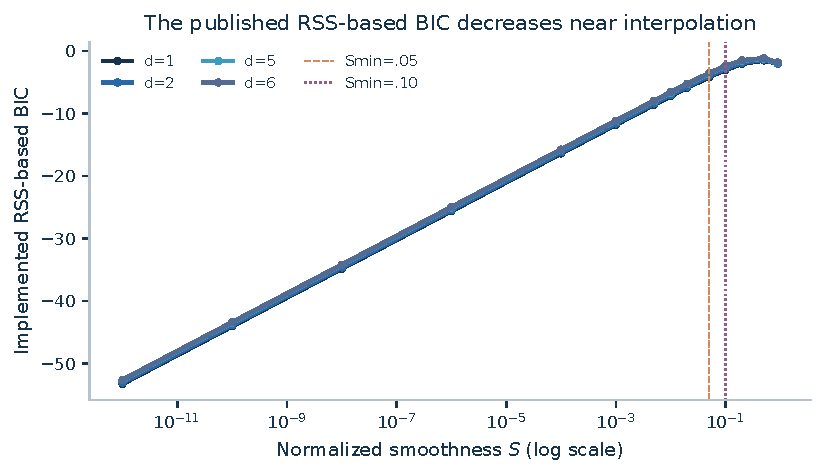
\includegraphics[width=\columnwidth]{figures/bic_boundary.pdf}
\caption{Residual-based BIC from the published equation on a small-$s$ grid for a seeded smooth-trend sample ($n=64$, fixed $\mu=0$). The curves decrease toward interpolation. Dashed and dotted lines mark the candidate restrictions used for sensitivity, not statistically optimal cutoffs.}
\label{fig:bic}
\end{figure}
